% !TeX root=main.tex
\chapter{تحقیقات و نوآوری‌های هوش مصنوعی در فرآوری مواد معدنی}

\section*{مقدمه}
فرآوری مواد معدنی یکی از بخش‌های کلیدی صنعت معدن است که هدف آن جداسازی مواد با ارزش از سنگ خام می‌باشد. 
این فرآیند شامل مراحلی نظیر خردایش، آسیاب، جدایش، فلوتاسیون، و آبگیری است. 
با توجه به هزینه‌های بالای انرژی، نوسانات کیفیت سنگ، و خطرات زیست‌محیطی، استفاده از فناوری‌های نوین مانند هوش مصنوعی می‌تواند منجر به افزایش بهره‌وری، کاهش هزینه‌ها، و ارتقای ایمنی شود. 

\begin{figure}[h!]
\centering
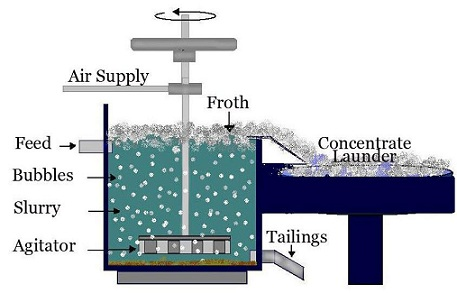
\includegraphics[width=0.8\textwidth]{images/mining_flow.jpg}
\caption{نمای کلی از فرآیند فرآوری مواد معدنی (خردایش، آسیاب، جدایش و آبگیری).}
\end{figure}

\section{آزمایشگاه تخصصی فرآوری مواد معدنی}

\subsection*{چالش‌های موجود}
در آزمایشگاه معمولاً باید نمونه را به دستگاه ببری و کلی زمان بگیرد. این فرآیند زمان‌بر و پرهزینه است.

\subsection*{نوآوری‌های هوش مصنوعی}

\subsubsection*{تشخیص ترکیب سنگ با عکس‌برداری}
با بینایی ماشین (AI) می‌توان از یک عکس میکروسکوپی یا حتی موبایل، رنگ، شکل و بافت سنگ را تحلیل کرد و حدس زد چه مقدار فلز داخل آن است. این روش سریع‌تر و کم‌هزینه‌تر از روش‌های سنتی است.

\subsubsection*{پیش‌بینی بهترین روش جداسازی}
در آزمایشگاه روش‌های مختلفی برای جدا کردن فلز وجود دارد (مثلاً شستشو با آب، مواد شیمیایی یا حرارت). AI می‌تواند با دیدن نتایج آزمایش‌های قبلی پیش‌بینی کند که کدام روش بیشترین بازده را می‌دهد.

\subsubsection*{تحلیل داده‌های آزمایشگاهی}
هوش مصنوعی می‌تواند داده‌های آزمایشگاهی (مثل درصد فلزات، شرایط دما و فشار، مصرف مواد شیمیایی) را تحلیل کند و الگوهای بهینه پیدا کند. مثلاً بعد از چند بار آزمایش، AI می‌فهمد که اگر سرعت همزن در فلوتاسیون ۲۰٪ کمتر باشد، بازیابی فلز بیشتر می‌شود.

\section{کارخانه پایلوت و صنعتی}

\subsection*{چالش‌های موجود}
\begin{itemize}
  \item ناپایداری کیفیت خوراک ورودی
  \item توقفات ناگهانی تجهیزات
  \item مصرف بالای انرژی و آب
\end{itemize}

\subsection*{نوآوری‌های هوش مصنوعی}

\subsubsection*{کنترل خودکار دستگاه‌ها}
کارخانه پر از دستگاه‌های آسیاب، جداکننده، پمپ و نوار نقاله است. سنسورها مدام دما، لرزش، سرعت و فشار را می‌خوانند. AI می‌تواند این داده‌ها را تحلیل کند و مثلاً بگوید سرعت آسیاب را کمی کم کن چون کیفیت خروجی افت کرده.

\subsubsection*{پیش‌بینی خرابی تجهیزات (نگهداری پیش‌بینانه)}
AI می‌تواند از روی صدای موتور یا لرزش یک دستگاه بفهمد که احتمالاً ۲ هفته دیگر خراب می‌شود و قبل از توقف کامل خط تولید، تعمیرش کنی.

\subsubsection*{بهینه‌سازی مصرف انرژی}
بعضی وقت‌ها تغییر کوچک در دما یا فشار می‌تواند مصرف برق را خیلی کم کند. AI می‌تواند بهترین تنظیمات را پیدا کند تا هم کیفیت خوب باشد هم هزینه کم.

\subsubsection*{کنترل کیفیت محصول}
وقتی فلز یا ماده فرآوری شده آماده می‌شود، AI می‌تواند با عکس‌برداری و اندازه‌گیری سریع بگوید آیا کیفیتش در محدوده استاندارد است یا نه.

\subsubsection*{تحلیل داده‌های پایلوت}
می‌شود داده‌های پایلوت را به AI داد تا الگوها را شناسایی کند و قبل از سرمایه‌گذاری بزرگ روی یک کارخانه صنعتی، بهترین روش را پیشنهاد بده. مثلاً AI پیش‌بینی کند «اگر فلوتاسیون با فلان ماده شیمیایی ادامه پیدا کند، در مقیاس صنعتی هزینه مواد مصرفی ۳۰٪ بیشتر می‌شود» → یعنی قبل از اینکه خرج میلیاردی شود، خطر دیده می‌شود.

\section{تجهیزات خط فرآوری}

هوش مصنوعی می‌تواند روی هر مرحله نظارت کند و بهترین شرایط را پیشنهاد بده. تجهیزات اصلی شامل:
\begin{itemize}
  \item سنگ‌شکن فکی و مخروطی \lr{→} برای خردایش اولیه سنگ
  \item آسیای گلوله‌ای و رادمیل \lr{→} برای خردایش نرم‌تر و رسیدن به پودر
  \item سلول فلوتاسیون ستونی و مکانیکی \lr{→} جداسازی کانی‌ها (مثلاً مس از باطله) با استفاده از حباب هوا
  \item مارپیچ همفری و میز لرزان \lr{→} برای جدایش ثقلی (بر اساس وزن مخصوص مواد)
  \item تیکنر و فیلتر پرس \lr{→} برای آب‌گیری و مدیریت باطله‌ها
\end{itemize}

\subsection{سنگ‌شکن (\lr{Crusher})}

\subsubsection*{چالش‌های اصلی}
\begin{itemize}
  \item فرسایش سریع فک‌ها و چکش‌ها \lr{→} هزینه بالا و توقف تولید
  \item تغییر ناگهانی سختی سنگ‌ها \lr{→} مصرف انرژی بیشتر یا شکستن تجهیزات
\end{itemize}

\subsubsection*{ایده‌های نوآورانه با AI}
\begin{itemize}
  \item \textbf{مدل پیش‌بینی هوشمند سختی سنگ:} استفاده از پردازش تصویر روی خوراک ورودی (قبل از ورود به سنگ‌شکن). قبل از خردایش، \lr{AI} عکس سنگ را می‌بیند و سختی را تخمین می‌زند \lr{→} تنظیم فشار و سرعت به صورت خودکار.
  \item \textbf{شنیدن صدای سنگ‌شکن (\lr{AI} صوتی):} از روی فرکانس صدا تشخیص می‌دهد کی سنگ غیرمعمول یا فلز وارد دستگاه شده \lr{→} هشدار فوری قبل از آسیب.
  \item \textbf{بهینه‌سازی شکل خوراک‌دهی:} با هوش مصنوعی جهت خوراک‌دهی اصلاح می‌شود تا توزیع یکنواخت سنگ باعث کاهش لرزش و افزایش عمر فک‌ها شود.
\end{itemize}

\begin{figure}[h!]
\centering
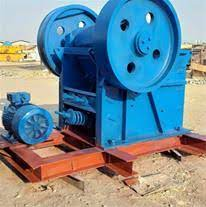
\includegraphics[width=0.6\textwidth]{images/crusher.jpg}
\caption{سنگ‌شکن فکی مورد استفاده در خردایش اولیه.}
\end{figure}

\subsection{آسیاب (\lr{Mill})}

\subsubsection*{چالش‌های اصلی}
\begin{itemize}
  \item مصرف وحشتناک انرژی
  \item گیرکردن یا بیش‌خردایش (\lr{Over-grinding}) \lr{→} اتلاف وقت و انرژی
\end{itemize}

\subsubsection*{ایده‌های نوآورانه با AI}
\begin{itemize}
  \item \textbf{بینایی ماشین برای تشخیص اندازه ذرات لحظه‌ای:} دوربین \lr{AI} روی خروجی آسیاب \lr{→} بلافاصله اندازه ذرات را تخمین می‌زند و سرعت آسیاب یا اندازه گلوله‌ها را تنظیم می‌کند.
  \item \textbf{بهینه‌سازی دینامیکی گلوله‌ها:} الگوریتم \lr{AI} محاسبه می‌کند چه ترکیبی از گلوله‌های کوچک/بزرگ بهترین بازدهی را دارد \lr{→} سفارش هوشمند گلوله برای خط تولید.
  \item \textbf{مدل‌سازی مصرف انرژی + کیفیت محصول:} با یادگیری تقویتی (\lr{Reinforcement Learning}) \lr{→} آسیاب یاد می‌گیرد چطور با کمترین انرژی، بهترین خروجی را بدهد.
\end{itemize}

\begin{figure}[h!]
\centering
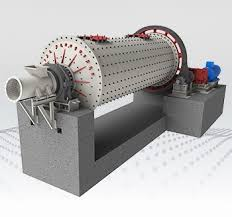
\includegraphics[width=0.6\textwidth]{images/mill.jpeg}
\caption{آسیاب گلوله‌ای در مدار فرآوری مواد معدنی.}
\end{figure}

\subsection{سلول فلوتاسیون (\lr{Flotation Cell})}

\subsubsection*{چالش‌های اصلی}
\begin{itemize}
  \item تغییر کیفیت سنگ → تنظیم دستی کف‌سازها و کلکتورها
  \item خطای انسانی زیاد در تشخیص "کیفیت کف"
\end{itemize}

\subsubsection*{ایده‌های نوآورانه با AI}
\begin{itemize}
  \item \textbf{بینایی ماشین برای آنالیز کف فلوتاسیون:} \lr{AI} از روی رنگ، شکل و پایداری کف، کیفیت فرآیند را تحلیل می‌کند \lr{→} بدون نیاز به اپراتور.
  \item \textbf{مدل‌های چندعاملی (\lr{Multi-agent AI}):} برای کنترل تزریق هوا، مواد شیمیایی و همزن به صورت همزمان \lr{→} یکپارچه‌سازی کل فرآیند.
  \item \textbf{مدل یادگیری از تجربه (\lr{Transfer Learning}):} اگر معدن \lr{A} روی سنگ مس کار کرده، تجربه مدل \lr{AI} برای معدن \lr{B} هم قابل استفاده باشد \lr{→} تسریع در تنظیمات.
\end{itemize}

\begin{figure}[h!]
\centering
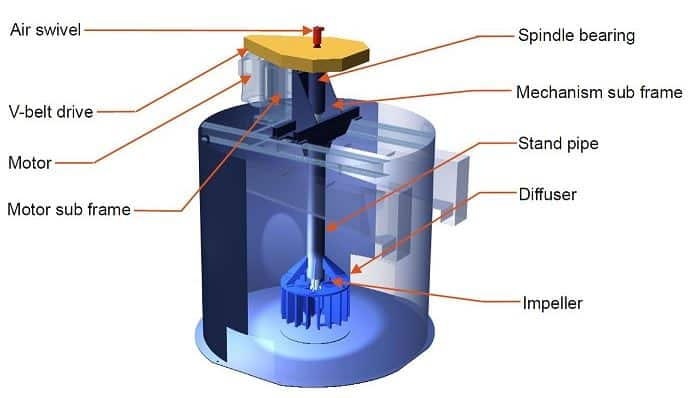
\includegraphics[width=0.6\textwidth]{images/flotation_cell.jpg}
\caption{سلول‌های فلوتاسیون مکانیکی برای جداسازی کانی‌ها.}
\end{figure}

\subsection{تجهیزات جدایش ثقلی (مارپیچ، میز لرزان)}

\subsubsection*{چالش‌های اصلی}
\begin{itemize}
  \item تغییر ناگهانی اندازه یا چگالی خوراک → افت کیفیت محصول
  \item وابستگی شدید به تجربه اپراتور
\end{itemize}

\subsubsection*{ایده‌های نوآورانه با AI}
\begin{itemize}
  \item \textbf{تشخیص لحظه‌ای مسیر حرکت ذرات:} با دوربین حرارتی یا \lr{RGB} \lr{→} \lr{AI} اصلاح زاویه مارپیچ یا میز را به‌صورت خودکار پیشنهاد می‌دهد.
  \item \textbf{ترکیب \lr{AI} با \lr{CFD} (شبیه‌سازی سیالات):} برای پیش‌بینی رفتار ذرات در شرایط مختلف خوراک \lr{→} تنظیم بهینه تجهیزات.
  \item \textbf{سیستم تطبیقی \lr{Real-time}:} میز لرزان یا مارپیچ به طور خودکار خودش را متناسب با خوراک ورودی تنظیم می‌کند.
\end{itemize}

\begin{figure}[h!]
\centering
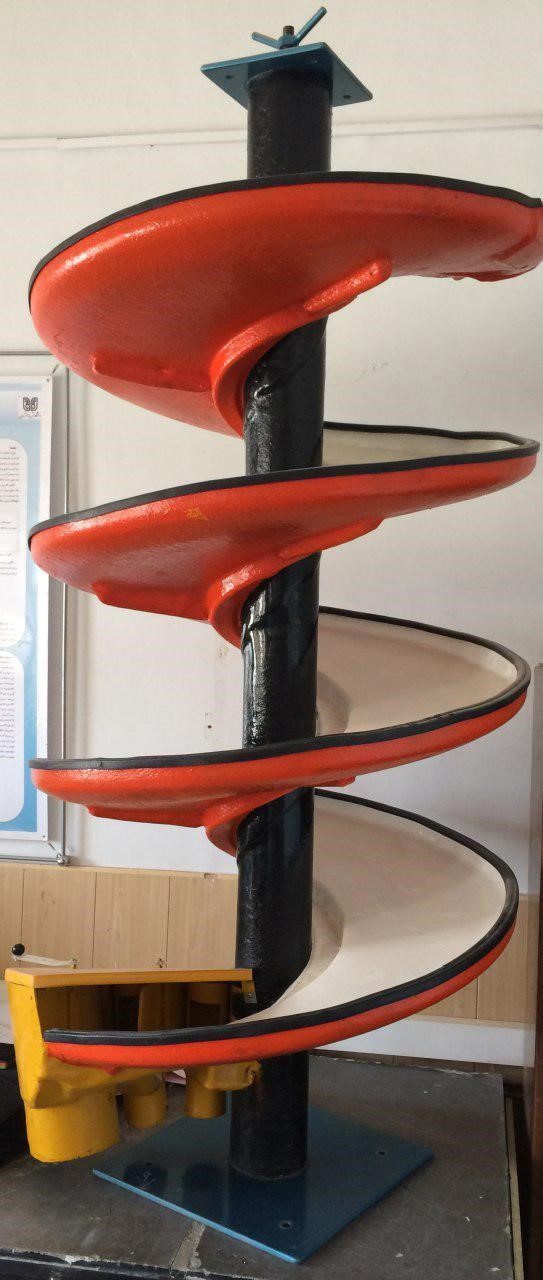
\includegraphics[width=0.6\textwidth]{images/gravity_separation.jpg}
\caption{میز لرزان برای جدایش ثقلی مواد معدنی.}
\end{figure}

\subsection{تیکنر و فیلتر پرس (\lr{Thickener \& Filter Press})}

\subsubsection*{چالش‌های اصلی}
\begin{itemize}
  \item بازیافت کم آب
  \item گرفتگی فیلترها و نیاز به شستشوی مکرر
  \item کیفیت پایین لجن
\end{itemize}

\subsubsection*{ایده‌های نوآورانه با AI}
\begin{itemize}
  \item \textbf{مدل \lr{AI} برای پیش‌بینی گرفتگی فیلتر:} از روی فشار، دما و جریان \lr{→} قبل از توقف خط.
  \item \textbf{بهینه‌سازی مصرف فلوکولانت:} \lr{AI} از روی کیفیت خوراک مقدار دقیق ماده شیمیایی را تعیین می‌کند.
  \item \textbf{مدل‌سازی ریسک سد باطله:} \lr{AI} از داده‌های خروجی تیکنر (غلظت لجن و دبی آب) استفاده می‌کند تا خطر تجمع بیش از حد یا ناپایداری سد را هشدار بدهد.
\end{itemize}

\begin{figure}[h!]
\centering
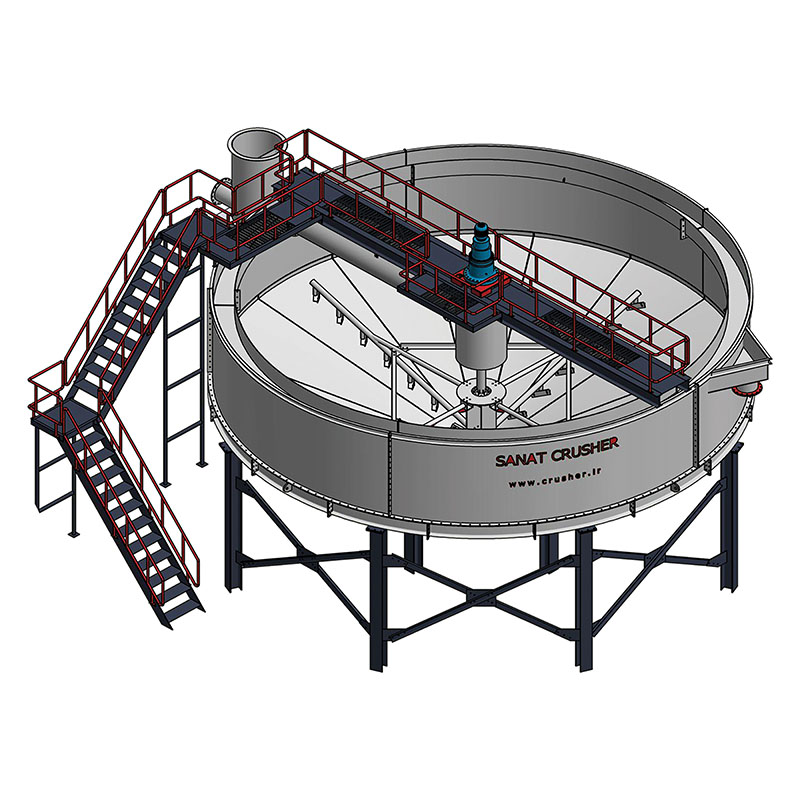
\includegraphics[width=0.6\textwidth]{images/thickener.jpg}
\caption{تیکنر صنعتی برای آبگیری و بازیافت آب.}
\end{figure}

\section*{جمع‌بندی}
کاربرد هوش مصنوعی در فرآوری مواد معدنی نه‌تنها باعث افزایش بازده و کاهش هزینه‌ها می‌شود، بلکه می‌تواند در ارتقای ایمنی و پایداری محیط‌زیستی نیز نقش کلیدی ایفا کند. 
این نوآوری‌ها مسیری نو برای حرکت معادن کشور به سمت معدن‌کاری هوشمند (\lr{Smart Mining}) فراهم می‌کنند.
